% Intended LaTeX compiler: pdflatex
\documentclass[11pt]{article}
\usepackage[utf8]{inputenc}
\usepackage[T1]{fontenc}
\usepackage{graphicx}
\usepackage{grffile}
\usepackage{longtable}
\usepackage{wrapfig}
\usepackage{rotating}
\usepackage[normalem]{ulem}
\usepackage{amsmath}
\usepackage{textcomp}
\usepackage{amssymb}
\usepackage{capt-of}
\usepackage{hyperref}
\author{Rodda John}
\date{06/22/2020}
\title{Functions}
\hypersetup{
 pdfauthor={Rodda John},
 pdftitle={Functions},
 pdfkeywords={},
 pdfsubject={},
 pdfcreator={Emacs 25.2.1 (Org mode N/A)}, 
 pdflang={English}}
\begin{document}

\maketitle

\section{Clerical Matters}
\label{sec:orge54ddd9}
\begin{itemize}
\item Welcome!
\item We're a large group:
\begin{itemize}
\item Use Zoom well!
\item Chatting!
\item Raising hands!
\item Faster / slower!
\end{itemize}
\end{itemize}
\subsection{Schedule}
\label{sec:org810c6bf}
\begin{center}
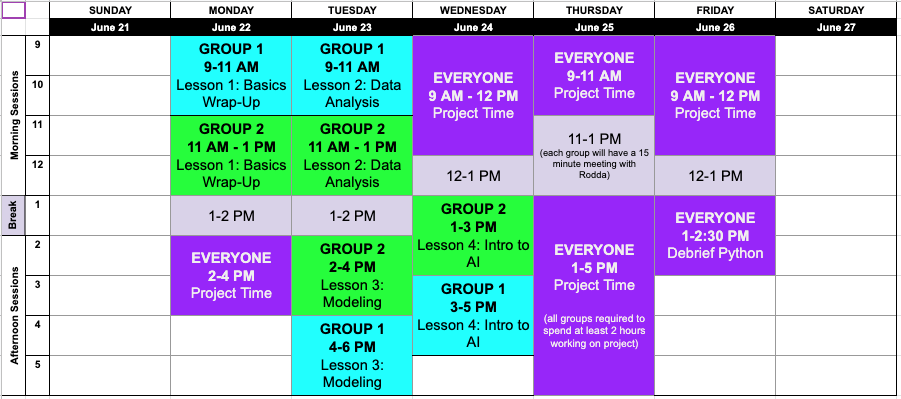
\includegraphics[width=.9\linewidth]{./src/schedule.png}
\end{center}
\subsection{Today}
\label{sec:orgbd2c795}
\begin{itemize}
\item Introduce you to writing your own functions
\item Learn about breaking projects down into manageable pieces
\item Start thinking algorithmically
\end{itemize}
\section{Functions}
\label{sec:orge21e2c7}
\begin{itemize}
\item What is a function?
\item A function is a procedure that execute code given certain inputs.
\item It must have
\begin{itemize}
\item A name
\item A definition (either local or in a library)
\end{itemize}
\item It may have
\begin{itemize}
\item Inputs (we will call these args, or arguments)
\item Outputs (we will call these return values)
\end{itemize}
\end{itemize}
\subsection{Why are these useful?}
\label{sec:org10fc933}
\begin{itemize}
\item Why are functions the most useful programming tool?
\item What are some use-cases?
\item How can we conceptualize a function?  How can we tell whether we ought make a function?
\end{itemize}
\section{Functions in Python}
\label{sec:org2efd88e}
\begin{itemize}
\item We need to learn how to do two things:
\begin{itemize}
\item Calling functions (executing them, using them)
\item Defining functions (making our own)
\end{itemize}
\end{itemize}
\subsection{Calling Functions}
\label{sec:org74f7a80}
\begin{verbatim}
print('Hello World!')
\end{verbatim}
\begin{verbatim}
len([1, 2, 3, 4, 5, 6])
\end{verbatim}
\begin{verbatim}
input()
\end{verbatim}
\begin{itemize}
\item How many \texttt{args} does each function have?
\item What is each functions output?
\end{itemize}
\subsection{Defining Functions}
\label{sec:org76f96a4}
\subsubsection{Simple Function}
\label{sec:orga453400}
\begin{itemize}
\item This function:
\begin{itemize}
\item Accepts two numerical inputs
\item Returns the product
\end{itemize}
\end{itemize}
\begin{verbatim}
def product(x, y):
    return x * y
\end{verbatim}
\subsubsection{Sum of a list}
\label{sec:org6c1f246}
\begin{itemize}
\item This function:
\begin{itemize}
\item Accepts a list
\item Returns the sum of the elements of the list
\end{itemize}
\end{itemize}
\begin{verbatim}
def sum_of_list(l):
    to_return = 0  # Tracks the sum of the list

    i = 0  # Iterator to iterate through the list

    while i < len(l):
	to_return += l[i]
	i = i + 1

    return to_return
\end{verbatim}
\subsubsection{Generally}
\label{sec:org1c72e37}
\begin{itemize}
\item \texttt{def} opens a function definition block
\item A name is required, as well as \texttt{()} to denote the args
\item Take note of the \texttt{:}
\item As with \texttt{if} statements, and \texttt{while} loops, the code in the function is indented
\end{itemize}
\subsubsection{Thus}
\label{sec:org3c9a5f4}
\begin{verbatim}
def <name>(<args>):
--> code
--> (optional) return <to_return>
\end{verbatim}
\section{Let's Try it Out}
\label{sec:org0ed9b42}
\subsection{First Problem}
\label{sec:orgfe4fa0e}
\begin{itemize}
\item Write a function (\texttt{sum}) that:
\begin{itemize}
\item Accepts two numerical inputs
\item Returns the sum
\end{itemize}
\item How can we test this function?
\begin{itemize}
\item What are the edge cases?
\end{itemize}
\end{itemize}
\subsubsection{First Problem Solution}
\label{sec:org0f75c49}
\begin{verbatim}
def sum(x, y):
    return x + y
\end{verbatim}
\begin{verbatim}
sum(1, 2)   # Should be 3
sum(4, -2)  # Should be 2
sum(4, 0)   # Should be 4
\end{verbatim}
\subsection{Second Problem}
\label{sec:org20fa6ba}
\begin{itemize}
\item Write a function (\texttt{product}) that:
\begin{itemize}
\item Accepts two numerical inputs
\item Returns the product
\item Does not use the \texttt{*} operator, and instead uses the \texttt{sum} function we defined above
\end{itemize}
\end{itemize}
\subsubsection{Second Problem Solution}
\label{sec:org09386eb}
\begin{verbatim}
def product(x, y):
    to_return = 0

    iterator = 0

    while iterator < y:
	to_return = to_return + x

	iterator = iterator + 1

    return to_return
\end{verbatim}
\begin{verbatim}
product(1, 2)   # Should be 2
product(100, 2) # Should be 200
product(2, 100) # Should be 200
product(2, .5)  # Should be 1
\end{verbatim}
\subsection{Third Problem}
\label{sec:orga6ed0b2}
\begin{itemize}
\item Write a function(\texttt{divisible\_by}) that:
\begin{itemize}
\item Accepts two numerical inputs (\texttt{number}, and \texttt{factor})
\item Returns true if and only if \texttt{number} is evenly divisble by \texttt{factor}
\item Recall the \texttt{\%} operator, which returns the remainder of the first operand by the second
\end{itemize}
\end{itemize}
\subsubsection{Third Problem Solution}
\label{sec:orgcaf45d2}
\begin{verbatim}
def divisible_by(number, factor):
    remainder = number % factor

    if remainder == 0:
	return True
    else:
	return False
\end{verbatim}
\begin{verbatim}
divisible_by(4, 2)  # Should be True
divisible_by(4, 1)  # Should be True
divisible_by(15, 3) # Should be True
divisible_by(15, 4) # Should be False
\end{verbatim}

\subsubsection{Or, even shorter}
\label{sec:org4aa6b5a}
\begin{verbatim}
def divisible_by(number, factor):
    remainder = number % factor

    if remainder == 0:
	return True
    return False
\end{verbatim}
\subsubsection{Or, even shorter}
\label{sec:org2b99f62}
\begin{verbatim}
def divisible_by(number, factor):
    return number % factor == 0
\end{verbatim}
\end{document}
